\onecolumn
\section*{Appendix A}
%%%%%%%%%%%%%%% begin table   %%%%%%%%%%%%%%%%
\begin{table}
\begin{center}
\caption[Industry standard and measured skateboard dimensions]{Industry standards and measured values from a PolarSkate Co. deck with Independent trucks}
\label{t_typical}
\begin{tabular}{l l l}
& & \\ % put some space after the caption
\hline
Description & Variable & Value \\
\hline
Wheel density (PU) & $\rho_{pu}$    & $1130 \quad [\frac{kg}{m^3}]$ \footnotemark\\
Hard maple density & $\rho_{maple}$ & $705 \quad [\frac{kg}{m^3}]$ \footnotemark\\
Thickness veneer & $d_{veneer}$ & $0.0016 \quad [m]$ \footnotemark\\
Specific mass PVA glue & $s_{glues}$ & $0.105 \quad [\frac{kg}{m^2}]$ $^{3}$  \footnotemark  \\
Density steel & $\rho_{steel} $ & $ 7700 \quad [\frac{kg}{m^3}] $ \\
Radius axle & $r_{axle} $   & $0.004 \quad [m] ^*$ \\
Width deck & $d_{D}$ & $0.21 \quad [m] ^*$ \\
Number of ply's & $n_{ply}$  & $7 $ \\
Mass bearing & $m_{bearing} $ & $0.012 \quad [kg] ^*$ \\ 
Mass truck   & $m_{truck} $   & $0.366 \quad [kg] ^*$ \\
\hline
\multicolumn{3}{l}{$^{1}$ \scriptsize{\url{https://www.lorkindustrias.com/}}} \\ 
\multicolumn{3}{l}{$^{2}$ \scriptsize{\url{https://www.wood-database.com/hard-maple/}}} \\ 
\multicolumn{3}{l}{$^{3}$ \scriptsize{\url{https://www.timberaid.com/}}} \\ 
\multicolumn{3}{l}{$^{4}$ \scriptsize{\url{http://www.franklinadhesivesandpolymers.com}}} \\ 
\multicolumn{3}{l}{$^{*}$ \scriptsize{Measured: caliper ($\pm 0.1mm$), scale ($\pm 1gram$)}} \\ 
\end{tabular}
\end{center}
\end{table}
%%%%%%%%%%%%%%%% end table %%%%%%%%%%%%%%%%%%%

\subsection*{Mesh example}
 By default each phase is subdivided into 10 mesh sections. Each mesh sections has 4 collocation points where the last of mesh section $n$ overlaps with the first collocation point of mesh section n+1 and so on. Thus each non beginning section has two overlapping points, this is the definition of the LGL method. This means by default each phase uses 31 collocation points. Mesh refinement is done when the mesh error did not reach the mesh tolerance. If the mesh section did not meet the tolerance, estimated $k$ extra collocation points are added to the mesh section. This means that the polynomial in the mesh section increased to the order $4+k$. This process will go on until the mesh tolerance is met or $k$ is estimated at a number that will exceed a 10th order polynomial. In this case the mesh section will be split up in new smaller sections. The sections will be split into parts that will match the expectation to 4 collocation points. For example, when the estimation of a 'correct' integration is estimated at 13 collocation points, the section will be split into four equally sized sections. When the estimation is to need 17 collocation points, 5 sections will be created. This method should be numerically efficient, since only the sections that show high nonlinearity and need a finer mesh will be integrated more thoroughly. If the tolerance is already met with a lower order integration, there will be no refinement\cite{rao_survey_2010,brockie_predictive_nodate,fasano_space_2016}. 

\section*{Mass, centre of mass and inertia model}


\section*{Inertia measurement}
To verify the inertial values obtained in the parameterized model of the skateboard, the inertia of two arbitrary skateboards are measured. 
\subsection*{Theory}
The skateboards inertia is measured by approximating the board as a compound pendulum. The inertia in a compound pendulum is directly related to the period of the swing of the pendulum. The torque produced by gravity is:
$$
\alpha I_o=-L m g \theta
$$
Using that the angular acceleration $(\alpha)$ can also be written as $\frac{d^2 \theta}{d t^2}$, we can re-write the angular acceleration as follows:
$$
\frac{d^2 \theta}{d t^2}=-\left(\frac{m g L}{I_o}\right) \theta
$$
This is a second order differential equation, for which we can use the standard solution for $\frac{d^2 \theta}{d t^2}=-b \theta$, which gives $\theta(t)=\cos (\omega t+\phi)$ with $\omega^2=b$. This results in an expression for the angular speed $(\omega)$ :
$$
\omega=\sqrt{\frac{m g L}{I_o}}
$$
Now that we can see the correlation between the period and the inertia of the compound pendulum, we can find the inertia about the COM of the skateboard by applying the parallel axis theorem:
\begin{equation}
    I_c = I_o + m L^2
\end{equation}
\subsection*{Method}
The skateboard was hung by ropes as seen in figure \ref{f_testsetup}. With a Silicon Sensing CRS43 gyroscope the rotational speed was measured. The skateboard was swung for 15 seconds released from 5, 10 or 15 degrees. The measured data was fit to a damped oscillation with a non linear least square method from SciPy. From the measured period the inertia values have been calculated giving the following fitted data shown in figure \ref{f_dampedoscillation}.
\begin{figure}
    \centering
    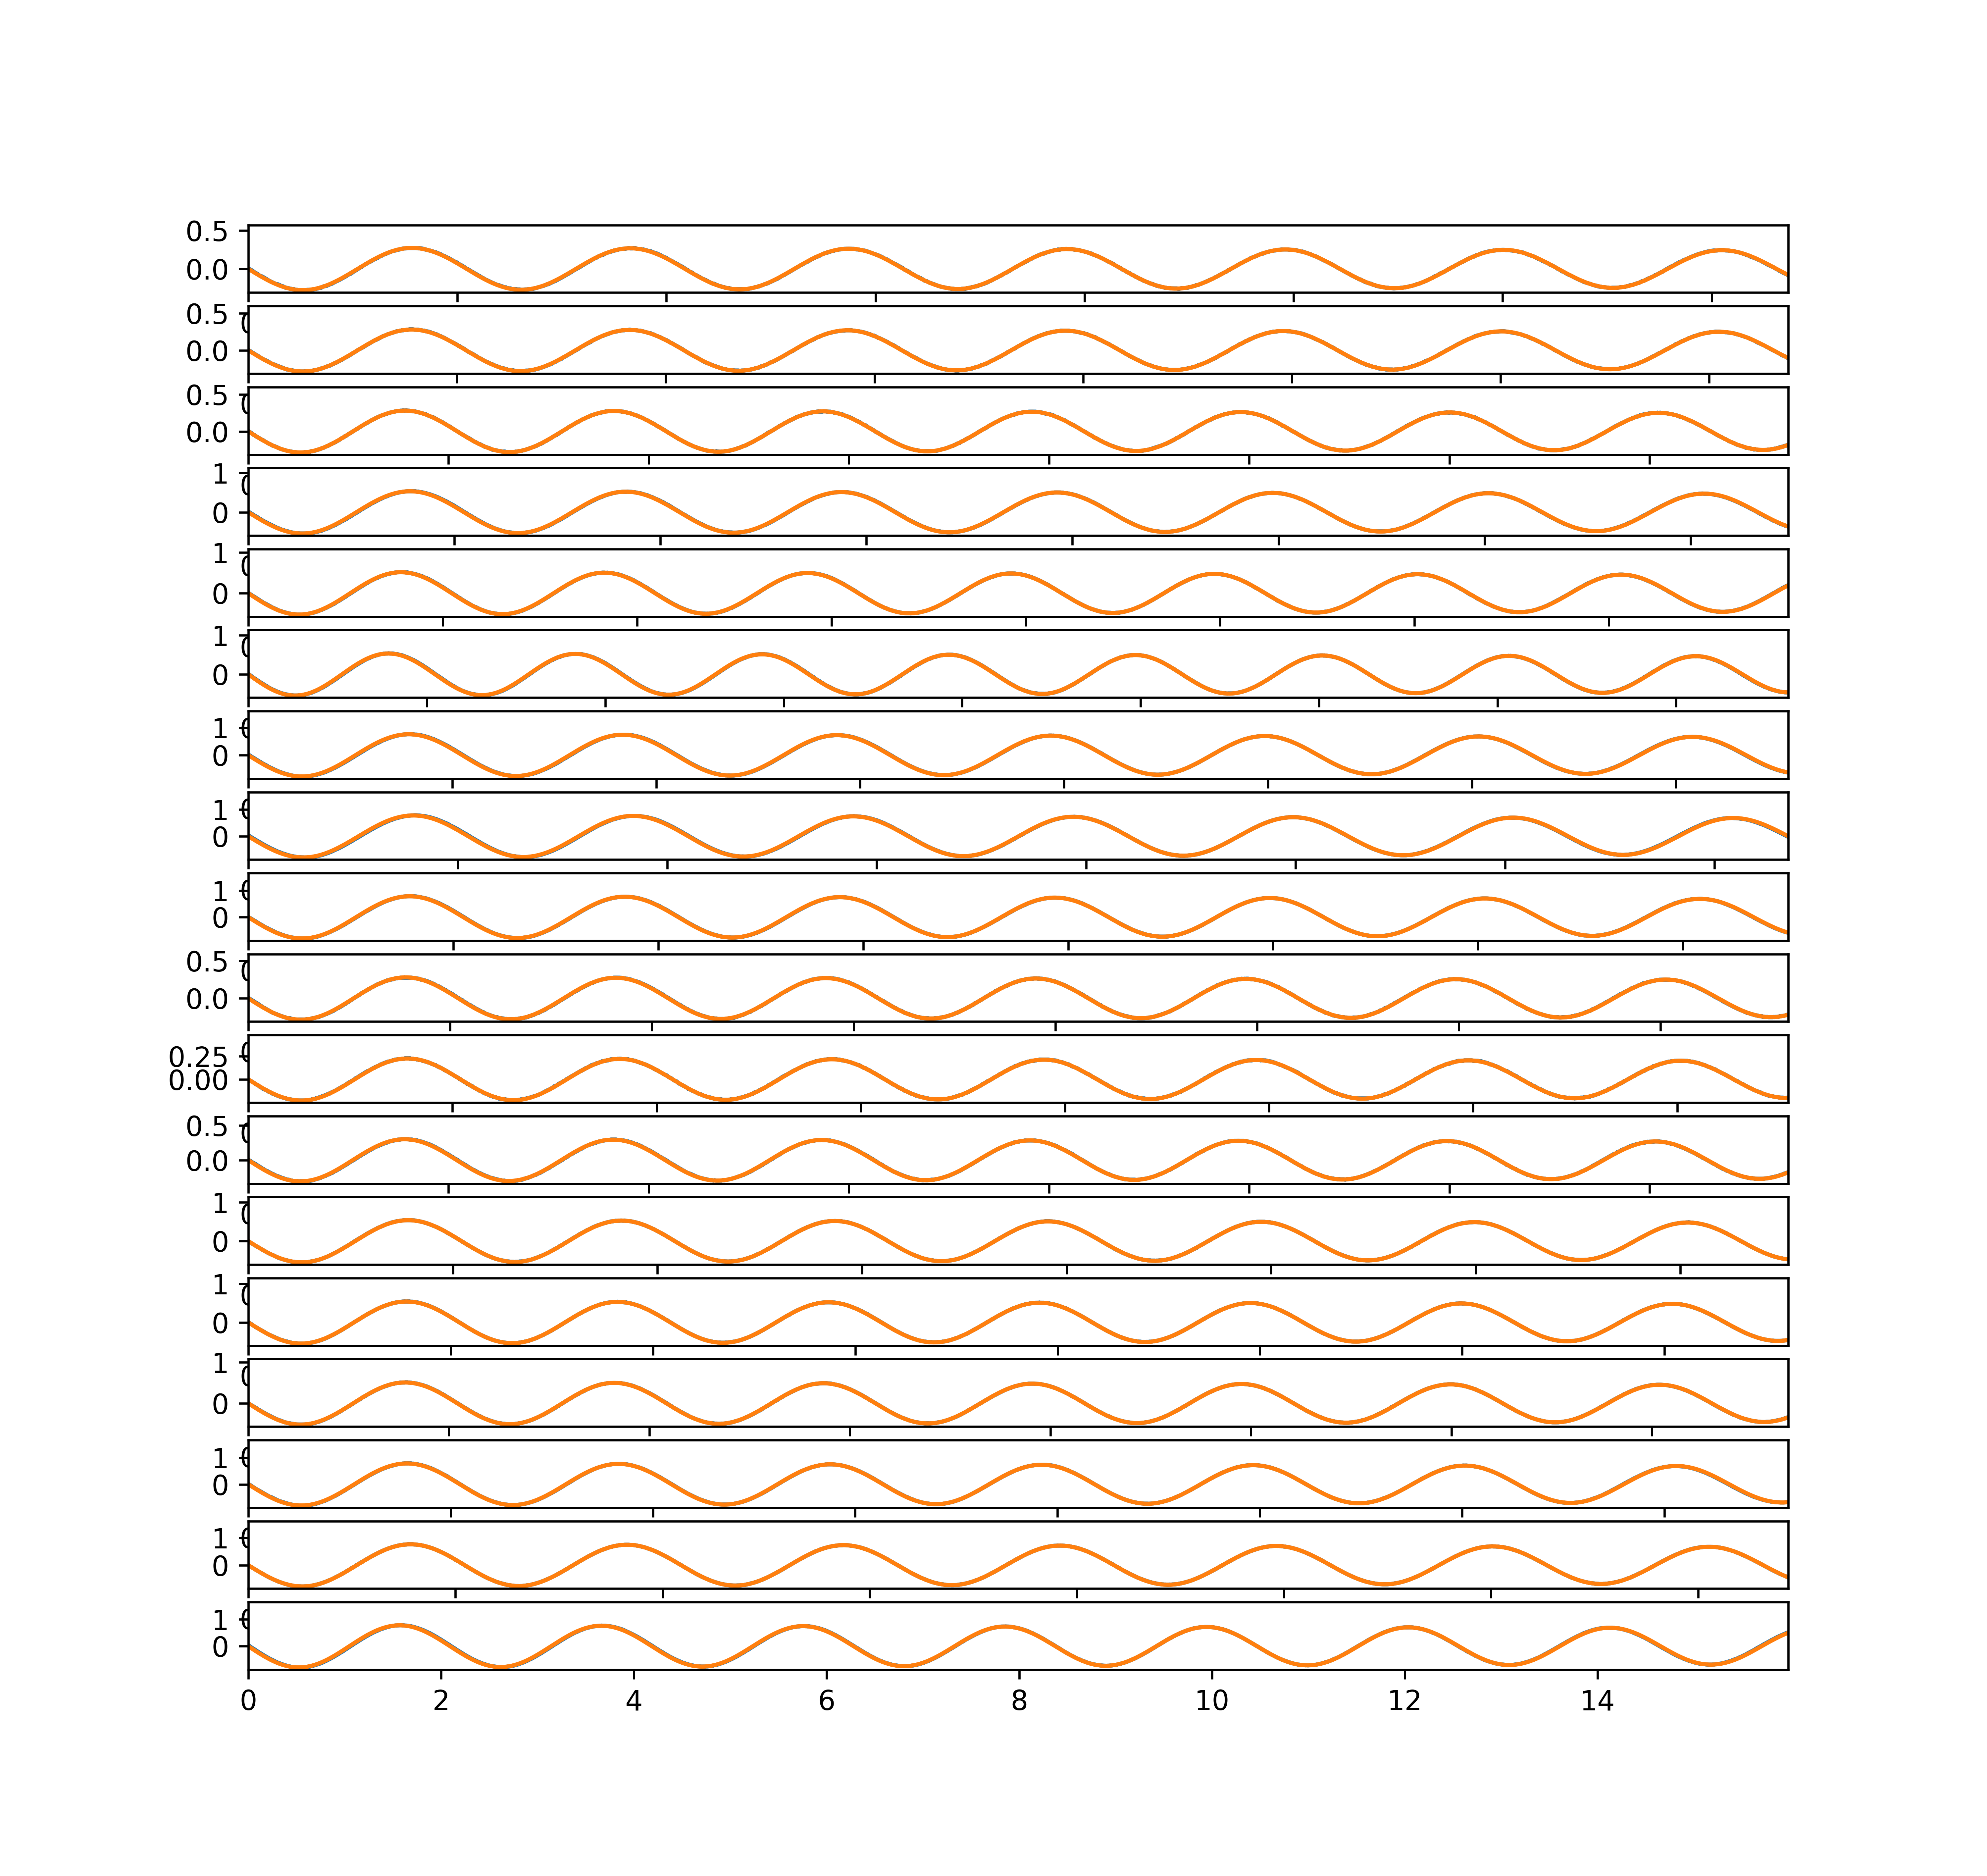
\includegraphics[width = 0.5\textwidth]{figure/damped_oscilation_fitdpi600.png}
    \caption{Fit of skateboard as compound pendulum}
    \label{f_dampedoscillation}
\end{figure}
The inertia results are given in figure \ref{f_inertianopower}
\begin{figure}
    \centering
    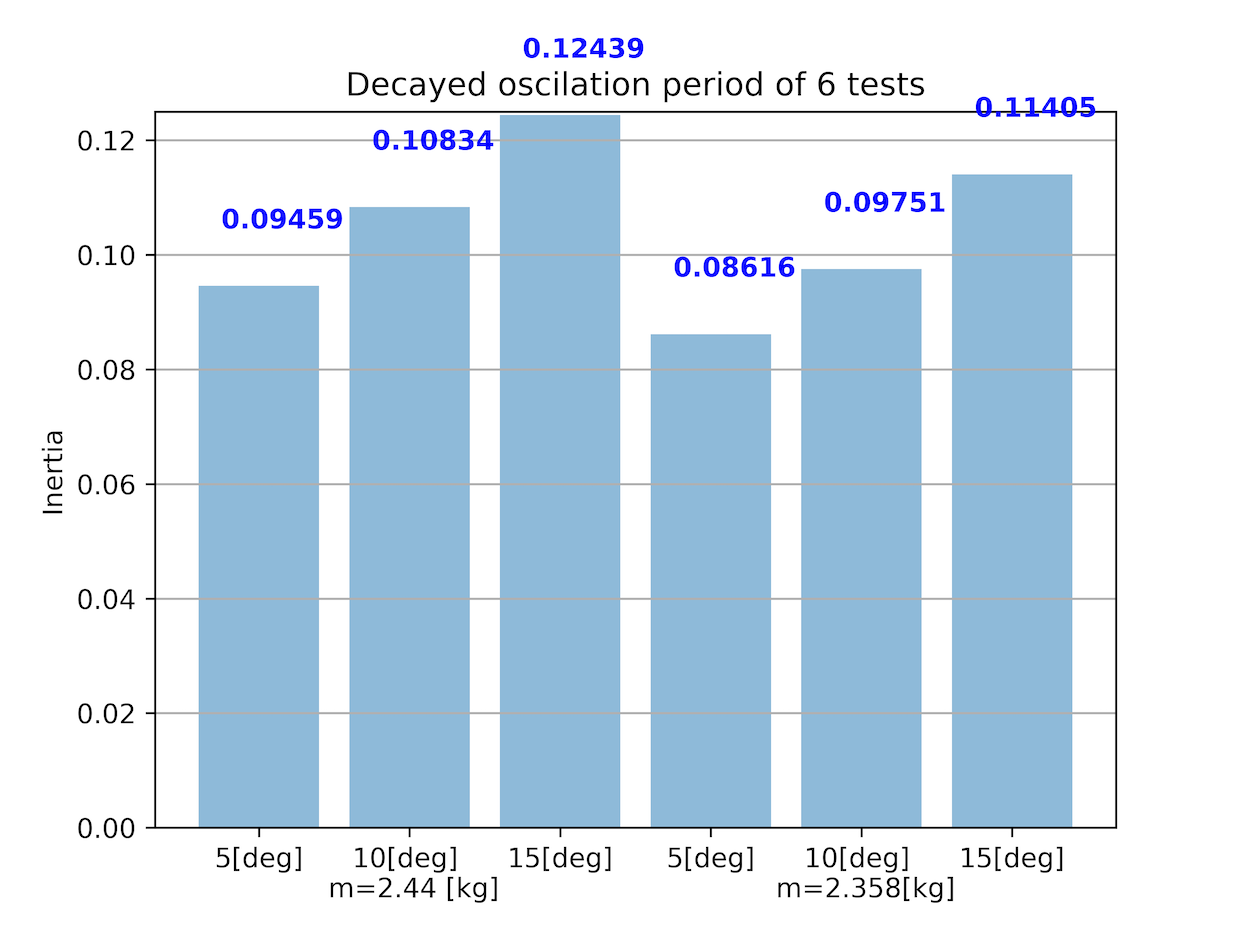
\includegraphics[width = 0.4\textwidth]{figure/Inertia_result_nopowerexpansiondpi600.png}
    \caption{Inertia results}
    \label{f_inertianopower}
\end{figure}
When it was clear that the inertia increased with an increase in starting angle, a power expansion is applied that accounts for small angle errors given by:
\begin{equation}
\begin{array}{r}
\omega_{exact} =  \approx T_0\left(1+\frac{1}{16} \theta^2+\frac{11}{3072} \theta^4+\frac{173}{737280} \theta^6\right. \\
\left.+\frac{22931}{1321205760} \theta^8+\ldots\right) .
\end{array}
\end{equation}
Which is used until the with precision $O^6$ results in the inertia data presented in figure \ref{f_powerexp}

\begin{figure}
    \centering
    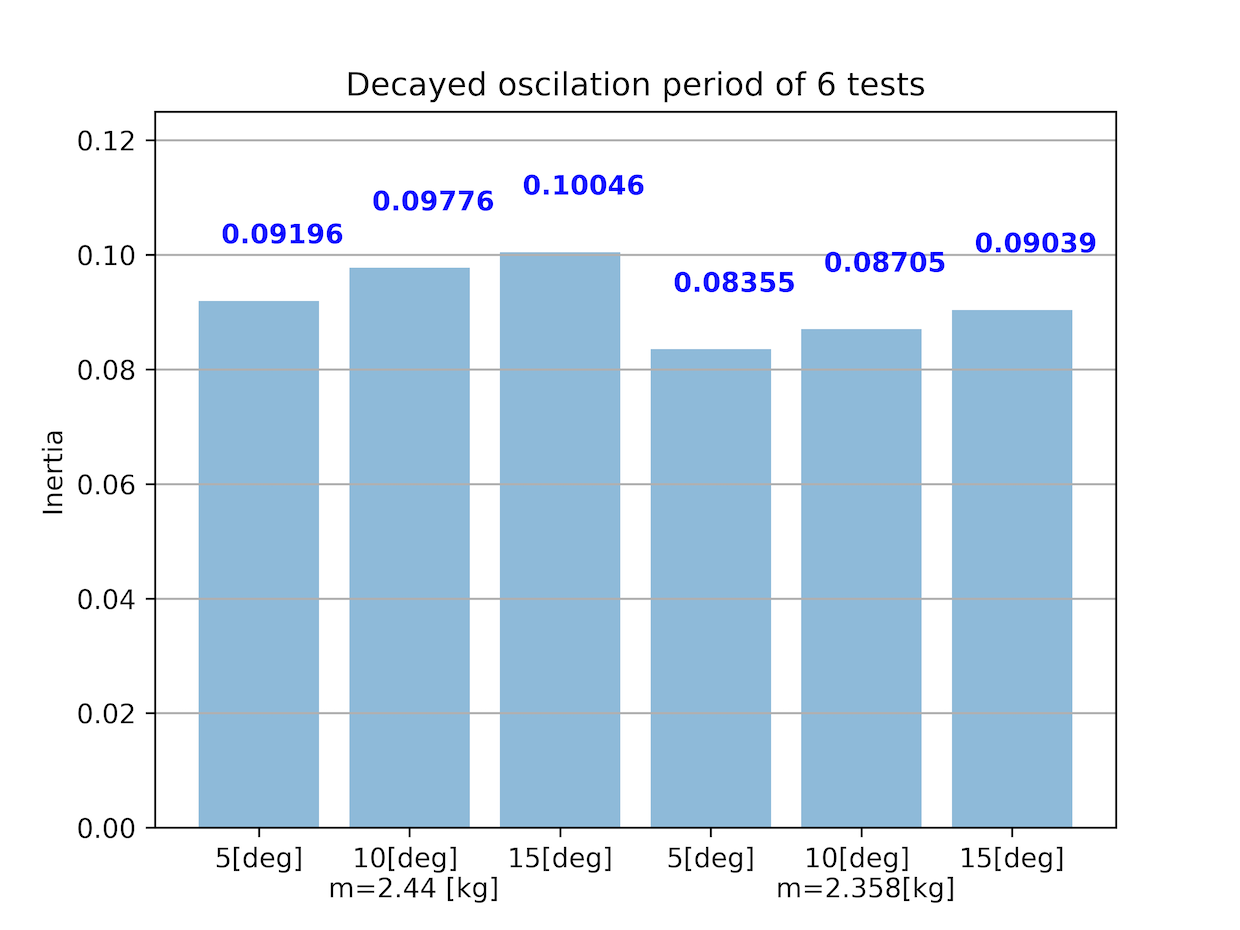
\includegraphics[width = 0.6\textwidth]{figure/Inertia_result_powerexpansiondpi600.png}
    \caption{Inertia result with power expansion}
    \label{f_powerexp}
\end{figure}

The calculated inertia value for skateboard with $m=2.44$ with the parameterized model is: 0.1219 [$kg\ m^2$]. The results show 0.09196 - 0.10046 [$kg\ m^2$]. The skateboards' inertia calculated with the parameterized model  with $m= 2.358$ is 0.1151 [$kg\ m^2$], while the results show 0.08355 - 0.09039 [$kg\ m^2$]. Both skateboards the model slightly overestimates the inertia.   The reduction in real life between the skateboards is 0.909\%, 0.890\%, 0.900\% between the different take off angles and different boards. In the parameterized model reduces inertia by 0.94 \%. This is of similar magnitude but needs more data to make it more exact. As a scaling approximation the parameter model is good enough.

\begin{figure}
    \centering
    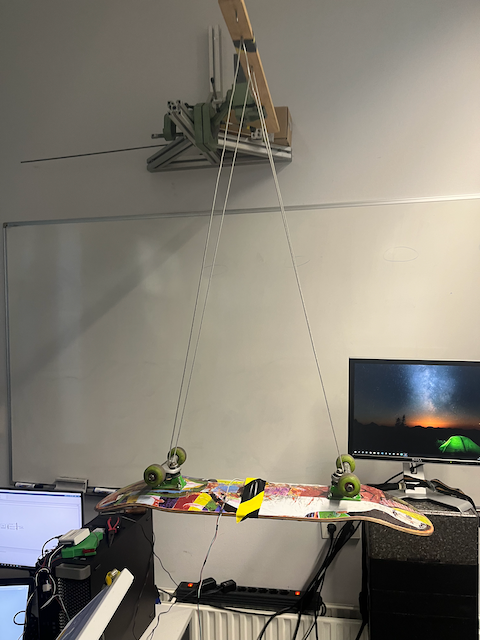
\includegraphics[width = 0.4 \textwidth]{figure/Testsetup.png}
    \caption{Test setup for inertia testing}
    \label{f_testsetup}
\end{figure}

\newpage
.
\newpage
\section*{Mass, centre of mass and inertia model}
\begin{verbatim}
    def Mass_model(width_deck, mass_bearing, mass_truck, height_truck, 
               height_truck0, width_wheel, n_ply, length_flat, length_tail, 
               radius_wheel, rho_pu, rho_maple, rho_steel, m_glue, 
               diameter_axle, d_veneer):

    mass_wheel = rho_pu * sm.pi * width_wheel * \
        ((2*radius_wheel)**2-diameter_axle**2) / 4  # V=pi*h*(D^2-d^2)/4

    mass_axle = sm.pi * (diameter_axle/2)**2 * width_deck * \
        rho_steel  # weight of axle, volume * steel * density

    #    _   _   ___________   _   _
    #  /  | | | |           | | | |  \
    # | 1 | |2| |     3     | |4| | 5 | 6=t1 7=w1 8=t2 9=w2
    #  \ _| |_| |___________| |_| |_ /

    #     1\                  /5
    #      2\_______3________/4
    #        6 \/         \/ 7
    #        8 O 9      10 O 11
    
    # Area of wooden components
    A1 = (1/2) * (1/4) * sm.pi * width_deck**2  # 1/4 pi d^2
    A2 = (length_tail - (width_deck/2)) * width_deck         # l * b
    A3 = length_flat * width_deck           # l * b
    A4 = A2
    A5 = A1
    
    thickness = n_ply*d_veneer
    dV = thickness*rho_maple+(m_glue/2*(n_ply-2))

    m1 = A1 * dV
    m2 = A2 * dV
    m3 = A3 * dV
    m4 = m2
    m5 = m1
    m6 = (mass_truck - mass_axle) * height_truck/height_truck0
    m7 = m6
    m8 = mass_axle
    m9 = 2*mass_wheel
    m10 = m8
    m11 = m9

    mass = [m1, m2, m3, m4, m5, m6, m7, m8, m9, m10, m11]
    return mass

def COM(mass, com_points, reference_point):
    # Function gets vector position from reference_point
    # Then assigns COM location to point COM
    # Returns position vector of COM points relative to COM
    r_m = []
    for i, x in enumerate(com_points):
        r_m.append(x.pos_from(reference_point)*mass[i])
    COM_skateboard = me.Point('COM_skateboard')
    COM_skateboard.set_pos(reference_point, (sum(r_m)/sum(mass)))
    return COM_skateboard
\end{verbatim}
\newpage
\begin{verbatim}
    
def Inertia_model(mass, com_points, com, majordim, shape):
    # Major dim:
    #   - (semi)cylinder;  diameter
    #   - cuboid: [l,h]
    #   - Triangle: [Base, Height]

    I_com = []
    I_steiner = []

    for i in range(len(mass)):
        if shape[i] == 'semicircle':
            I_com.append(((1/4)-(16/(9*sm.pi**2)))*mass[i]*(majordim[i]/2)**2)

        if shape[i] == 'cuboid':
            I_com.append((mass[i]/12) * (majordim[i]
                         [0]**2 + majordim[i][1]**2))

        if shape[i] == 'triangle':
            s = sm.sqrt((majordim[i][0]/2)**2+majordim[i][1]**2)
            beta = 2*sm.asin((majordim[i][0]/2)/s)
            I_com.append((mass[i]/2)*s**2*(1-(2/3)*sm.sin(beta)))

        if shape[i] == 'cylinder':
            I_com.append((1/2)*mass[i]*(majordim[i]/2)**2)
        #Trigsimp was sometimes necesarry due to a theta still being in there
        I_steiner.append(sm.trigsimp(mass[i]*d2s(sm.sqrt(com_points[i].\
        pos_from(com).dot(A.x)**2+com_points[i].pos_from(com).dot(A.y)**2)**2)))
    I_tot = sum(I_com)+sum(I_steiner)
    return I_tot, I_com, I_steiner
\end{verbatim}
